\documentclass[cs4size,a4pape,UTF8]{ctexart}   
%==================== 数学符号公式 ============
\usepackage{amsmath}                 % AMS LaTeX宏包
\usepackage[style=1]{mdframed}
\usepackage{amsthm}
\usepackage{amsfonts}
\usepackage{mathrsfs}                % 英文花体字 体
\usepackage{bm}                      % 数学公式中的黑斜体
\usepackage{bbding,manfnt}           % 一些图标,如 \dbend
\usepackage{lettrine}                % 首字下沉,命令\lettrine
\usepackage{url}
\def\attention{\lettrine[lines=2,lraise=0,nindent=0em]{\large\textdbend\hspace{1mm}}{}}
\usepackage{longtable}
\usepackage[toc,page]{appendix}
\usepackage{geometry}                % 页边距调整
\geometry{top=3.0cm,bottom=2.7cm,left=2.5cm,right=2.5cm}
%====================公式按章编号==========================
\usepackage{enumerate}
\numberwithin{equation}{section}
\numberwithin{table}{section}
\numberwithin{figure}{section}
%================= 基本格式预置 ===========================
\usepackage{fancyhdr}
\pagestyle{fancy}
\fancyhf{}  
\fancyhead[C]{\zihao{5}  \kaishu Beijing University of Posts and Telecommunications}
\fancyfoot[C]{~\zihao{5} \thepage~}
\renewcommand{\headrulewidth}{0.65pt} 
\CTEXsetup[format={\centering\bfseries\zihao{2}}]{section}
\CTEXsetup[nameformat={\bfseries\zihao{3}}]{subsection}
\CTEXsetup[nameformat={\bfseries\zihao{4}}]{subsubsection}
%================== 图形支持宏包 =========================
\usepackage{subfigure}
\usepackage{graphicx}                % 嵌入png图像
\usepackage{color,xcolor}            % 支持彩色文本、底色、文本框等
\usepackage{hyperref}                % 交叉引用
\usepackage{caption}
\captionsetup{figurewithin=section}
%==================== 源码和流程图 =====================
\usepackage{listings}                % 粘贴源代码
\usepackage{xcolor}
\usepackage{color}
\definecolor{dkgreen}{rgb}{0,0.6,0}
\definecolor{gray}{rgb}{0.5,0.5,0.5}
\definecolor{mauve}{rgb}{0.58,0,0.82}
 \usepackage{xcolor}
 \lstset{
  %行号
    numbers=left,
    %背景框
    framexleftmargin=8mm,
    frame=none,
     %背景色
    %backgroundcolor=\color[rgb]{1,1,0.76},
     backgroundcolor=\color[RGB]{245,245,244},
     %样式
   keywordstyle=\bf\color{blue},
   identifierstyle=\bf,
    numberstyle=\color[RGB]{0,192,192},
    commentstyle=\it\color[RGB]{0,96,96},
   stringstyle=\rmfamily\slshape\color[RGB]{128,0,0},
   %显示空格
    showstringspaces=false
 }


%--------------------
\hypersetup{hidelinks}
\usepackage{booktabs}  
\usepackage{shorttoc}
\usepackage{tabu,tikz}
\usepackage{float}

\usepackage{multirow}



\tabcolsep=1ex
\tabulinesep=\tabcolsep
\newlength\tikzboxwidth
\newlength\tikzboxheight
\newcommand\tikzbox[1]{%
        \settowidth\tikzboxwidth{#1}%
        \settoheight\tikzboxheight{#1}%
        \begin{tikzpicture}
        \path[use as bounding box]
                (-0.5\tikzboxwidth,-0.5\tikzboxheight)rectangle
                (0.5\tikzboxwidth,0.5\tikzboxheight);
        \node[inner sep=\tabcolsep+0.5\arrayrulewidth,line width=0.5mm,draw=black]
                at(0,0){#1};
        \end{tikzpicture}%
        }

\makeatletter
\def\hlinew#1{%
  \noalign{\ifnum0=`}\fi\hrule \@height #1 \futurelet
   \reserved@a\@xhline}
   
\newcommand{\tabincell}[2]{\begin{tabular}{@{}#1@{}}#2\end{tabular}}%

\usepackage{subfigure}

\usepackage{CJK}
\usepackage{ifthen}


\usepackage{graphicx} 
\newcommand{\HRule}{\rule{\linewidth}{0.5mm}}

\newtheorem{Theorem}{定理}
\newtheorem{Lemma}{引理} 
%%使得公式随章节自动编号
\makeatletter
\@addtoreset{equation}{section}
\makeatother
\renewcommand{\theequation}{\arabic{section}.\arabic{equation}}

%-------------------------
	
\usepackage{pythonhighlight}
\usepackage{tikz}                    
\usepackage{tikz-3dplot}
\usetikzlibrary{shapes,arrows,positioning}
%===================   正文开始    ===================
\begin{document}
\bibliographystyle{gbt7714-2005}     %论文引用格式
%===================  定理类环境定义 ===================
\newtheorem{example}{例}              % 整体编号
\newtheorem{algorithm}{算法}
\newtheorem{theorem}{定理}            % 按 section 编号
\newtheorem{definition}{定义}
\newtheorem{axiom}{公理}
\newtheorem{property}{性质}
\newtheorem{proposition}{命题}
\newtheorem{lemma}{引理}
\newtheorem{corollary}{推论}
\newtheorem{remark}{注解}
\newtheorem{condition}{条件}
\newtheorem{conclusion}{结论}
\newtheorem{assumption}{假设}
%==================重定义 ===================
\renewcommand{\contentsname}{目录}     
\renewcommand{\abstractname}{摘要} 
\renewcommand{\refname}{参考文献}     
\renewcommand{\indexname}{索引}
\renewcommand{\figurename}{图}
\renewcommand{\tablename}{表}
\renewcommand{\appendixname}{附录}
\renewcommand{\proofname}{证明}
\renewcommand{\algorithm}{算法} 
%============== 封皮和前言 =================
\begin{titlepage}

\begin{center}


% Upper part of the page

\includegraphics[width=0.65\textwidth]{figure/logo}\\[1cm]    

\textsc{\Large 论文}\\[0.5cm]


% Title
\HRule \\[1.5cm]
{ \huge \bfseries 形式化分析介绍}\\[0.94cm]
\HRule \\[1.5cm]

% Author and supervisor
\begin{minipage}{0.4\textwidth}
\begin{flushleft} \large
\emph{姓名: }
 \textsc{冯皓楠}\\
\end{flushleft}
\end{minipage}
\begin{minipage}{0.4\textwidth}
\begin{flushleft} \large

\end{flushleft}

\end{minipage}

\vfill

% Bottom of the page
{\large \today}

\end{center}

\end{titlepage}


%%=============设计(论文)任务书===========
%\begin{center}
%\zihao{-2}\textbf{\songti 本科生毕业设计(论文)任务书} 
%\end{center}
%\smallskip
%\renewcommand{\arraystretch}{1.3}
%\begin{tabular}{lll}
%\zihao{4} \textbf{\songti 学生姓名: 曹宇} & & \zihao{4} \textbf{\songti 专业班级:\quad\quad 船海1006班} \\ 
%\zihao{4} \textbf{\songti 指导教师:徐海祥}&\makebox [3cm] & \zihao{4} \textbf{\songti 工作单位:\quad 武汉理工大学} \\ 
%\end{tabular}\\
%\begin{tabular}{lll}
%\zihao{4} \textbf{\songti 设计(论文)题目:}& \zihao{4} \textbf{\songti  武汉理工本科论文\LaTeX 模板 } &\\ 
%\zihao{4} \textbf{\songti 设计(论文)主要内容:} \\
%\end{tabular} \\ 
%\begin{enumerate}
%\item \LaTeX 环境的配置
%\item 主要字体的控制和数学公式的选用
%\item 图表和代码的粘贴
%\end{enumerate}
%\begin{tabular}{ll}
%\zihao{4} \textbf{\songti 要求完成的主要任务:}
%\end{tabular} \\ 
%\begin{enumerate}
%\item 选择合适的\TeX 编辑系统
%\item 学习如何使用控制代码完成排版
%\item 合理的安排学习和科研的时间来发展自己兴趣爱好
%\end{enumerate}
%\begin{tabular}{ll}
%\zihao{4} \textbf{\songti 必读参考资料:}
%\end{tabular}
%\begin{enumerate}
%\item \LaTeX  \quad User Manual
%\item  字体设计的艺术
%\end{enumerate}
%\begin{tabular}{lll}
%\zihao{4} \textbf{\songti 指导教师签名: }&\makebox [4cm]& \zihao{4} \textbf{\songti 系主任签名:} \\
%& & \zihao{4} \textbf{\songti 院长签名(章)}
%\end{tabular}
%\thispagestyle{empty}
%\clearpage
%%==========本科生毕业设计(论文)开题报告  =============
%\begin{center}
%\zihao{-2} \textbf{\songti 武汉理工大学}\\
%\zihao{-2} \textbf{\songti 本科生毕业设计(论文)开题报告} 
%\end{center}
%\begin{tabular}{|l|}
%\hline \rule[-2ex]{0pt}{5.5ex} \makebox[13.5cm][l]{\zihao{4} \heiti 1、目的及意义(含国内外的研究现状分析) } \\ 
%\quad \LaTeX 是国际通行的科技论文排版软件,国际上科研机构和大学都采用它写作\\
%\quad 国内著名高校都有自己的本科生\LaTeX 模板供毕业生使用\\
%\quad 但是武汉理工大学还没有本科生\LaTeX 模板可以参考\\
%\quad 人类的价值在于创造而不是索取 \\
%\hline \rule[-2ex]{0pt}{5.5ex}  \zihao{4} \heiti
%2、基本内容和技术方案\\ 
%\quad 采用GITHUB托管降低代码维护成本\\
%\quad 加入在线\TeX 编辑器的使用简介 \\
%\quad 授人以渔,注重方法和理念的引导\\
%\hline \rule[-2ex]{0pt}{5.5ex}  \zihao{4} \heiti
%3、进度安排 \\ 
%\quad 离 deadline 两个月吃喝玩乐 \\
%\quad 离 deadline 一个月吃喝玩乐 \\
%\quad 离 deadline 半个月吃喝玩乐 \\
%\quad 离 deadline 一个星期狂写论文 \\
%\hline \rule[-2ex]{0pt}{5.5ex} \zihao{4} \heiti
%4、指导教师意见 \\ 
%\quad 曹宇同学是个好同志\\
%\quad 曹宇同志是个好同学\\
%\quad 本表格是支持跨页的长表格,你可以复制上面的内容进行测试\\
%\quad 具体方法是将tabular改为 longtable然后再编译\\
%\makebox[10cm][r]指导教师签名:\\
%\makebox[12cm][r]\quad 年\quad 月\quad 日\\
%\hline 
%\end{tabular} 
%\thispagestyle{empty}

\pagestyle{plain}
\pagenumbering{Roman}

\section*{\zihao{2} \centering \textbf{摘要} }

\vskip0.5cm

形式化方法是基于数学的特种技术,适合于验证和设计。形式化方法适用的领域非常多,除了在数学领域的机器证明,形式化方法还可以应用在计算机领域的硬件与软件验证,安全协议领域的协议验证与协议设计。将形式化方法用于软件和硬件设计,是期望能够像其它工程学科一样,使用适当的数学分析以提高设计的可靠性和鲁棒性。将形式化应用于安全协议分析,通过数学的手段可以发现人无法发现的协议漏洞,还可以证明协议在某些方面的安全性。

本文综合了与形式化、形式化方法、形式化分析、形式化验证有关的论文与网络资源内容,对与形式化应用的领域做了简单的介绍,并详细总结了形式化方法在安全协议领域的应用与方法。

\textbf{关键词:}  形式化方法,形式化验证, 安全协议 的形式化分析 


\addcontentsline{toc}{section}{摘要}





\clearpage
\pagestyle{empty}
\tableofcontents 
\thispagestyle{empty}
%============== 论文正文   =================
\pagestyle{fancy}
\newpage
\pagenumbering{arabic}%开始数字目录
\section{介绍}
 本章用于介绍与形式化有关的名词含义。
 
\subsection{形式化方法(Formal Methods)}
形式化方法是将概念或方法,经过高度抽象后使用一定的数学模型进行表示。之后,通过程式化的推演和计算来研究该数学模型,进而揭示概念和方法内在规律的一种研究方法。

形式化方法简单的说就是用数学工具进行定义、开发和验证(specification, development and verification)。数学家们认为,不论硬件还是软件工程,就像世间万物一样,所有的学问一样,归根结底是数学问题。''一个不懂数学的工程师不是一个好工程师''。如果所有的设计开发都能够按照严格的数学方法进行,那么开发出来的系统就会像数学本身一样的完美:软件不会出错,硬件永远正常。当然,这是数学家的理想。

来自维基百科(Formal method):在计算机科学中,特别是软件工程和硬件工程中,形式化方法是一种特殊的基于数学的技术,用于软件和硬件系统的规范、开发和验证。软件和硬件设计的形式化方法的产生于使用是由于用户对安全性不断上涨的期望导致的,像在其他同城学科一样,执行适当的数学分析可以提高设计系统的可靠性和健壮性。

In computer science, specifically software engineering and hardware engineering, formal methods are a particular kind of mathematically based techniques for the specification, development and verification of software and hardware systems. The use of formal methods for software and hardware design is motivated by the expectation that, as in other engineering disciplines, performing appropriate mathematical analysis can contribute to the reliability and robustness of a design.

Formal methods are best described as the application of a fairly broad variety of theoretical computer science fundamentals, in particular logic calculi, formal languages, automata theory, discrete event dynamic system and program semantics, but also type systems and algebraic data types to problems in software and hardware specification and verification\cite{formalmethods}.

当代著名逻辑学家鲍亨斯基认为:"形式化方法是这样一种方法,它完全撇开符号本身的意义,而根据某些只涉及符号书面形态的转换规则来进行符号操作的方法。

理解''形式化方法''时,注意区分与软件形式化方法(软件可靠性方法),因为形式化方法在软件工程领域的应用比较广泛,所以形式化方法往往指代软件形式化方法,即软件工程中的形式化设计与形式化验证等。


\subsection{形式化规范}
形式化规范就是用一套基于明确定义的数学概念的符号来书写,并且通常伴随着支持性的解释(非形式化)语句。这些数学概念被用来定义符号的句法和语义,以及支持逻辑推理的证明规则。支持形式化符号的句法和语义规则应该定义如何明确地识别其结构和确定其含义。并且必须有证据表明矛盾不可能产生,支持符号的所有规则都有定义或者引用。

\subsection{形式化语言}
使用的是以数学、数理逻辑符号语言为蓝本的科学语言,也称为"形式化语言"。它的基本特征是:语言保持单一性、无岐义性和明确性。形式化语言的推广运用作为一种用于研究手段,被称为形式化方法。

\subsection{形式化验证(Formal Verification)}
形式化验证(又叫形式化证明),在数学,计算机科学,人工智能领域都得到了广泛的应用。形式化的概念最早出现在数学界,又称为机器证明。

CertiK(一个用形式化验证为智能合约和区块链应用提供安全性服务的公司)的创始人顾荣辉用简洁的语句来描述形式化验证:用逻辑语言来描述规范,通过严谨的数学推演来检查给定的系统是否满足要求。

来自维基百科(Formal Verification):在硬件和软件系统中,形式化验证是通过形式化的数学方法来证明一个系统潜在算法的正确性行为或否定一个系统潜在算法的正确性行为。形式化验证可以帮助证明系统的正确性,例如:加密协议、组合电路、带有内部内存的数字电路,以及源代码形式表示的软件。对于这些系统的验证是通过对系统的抽象数学模型的形式化证明、数学模型与系统的性质之间的对应关系来实现的。通常用于建模系统的数学对象有有限状态机、标记转换系统、向加法系统、自动机、过程代数、编程语言的形式化语义等。

In the context of hardware and software systems, formal verification is the act of proving or disproving the correctness of intended algorithms underlying a system with respect to a certain formal specification or property, using formal methods of mathematics.

Formal verification can be helpful in proving the correctness of systems such as: cryptographic protocols, combinational circuits, digital circuits with internal memory, and software expressed as source code.

The verification of these systems is done by providing a formal proof on an abstract mathematical model of the system, the correspondence between the mathematical model and the nature of the system being otherwise known by construction. Examples of mathematical objects often used to model systems are: finite state machines, labelled transition systems, Petri nets, vector addition systems, timed automata, hybrid automata, process algebra, formal semantics of programming languages such as operational semantics, denotational semantics, axiomatic semantics and Hoare logic\cite{formalverification}.

\newpage
\section{形式化方法在不同领域的应用}
形式化方法的应用主要如下:

\begin{itemize}
\item 安全模型
\item 流分析
\item 安全协议分析
\item 软件验证
\item 硬件验证
\item 体系结构分析
\item 秘密信道分析
\end{itemize}

\subsection{数学领域的形式化}
数学领域,形式化的工作主要在于机器验证数学定理。
定理证明器包含Coq、Z3、CVC4、Vampire、E、Spass、Isabelle证明器等。以下是一个在Isabelle定理证明器中,关于质数的平方根不是有理数的证明:

\begin{figure}[thbp!]
\centering
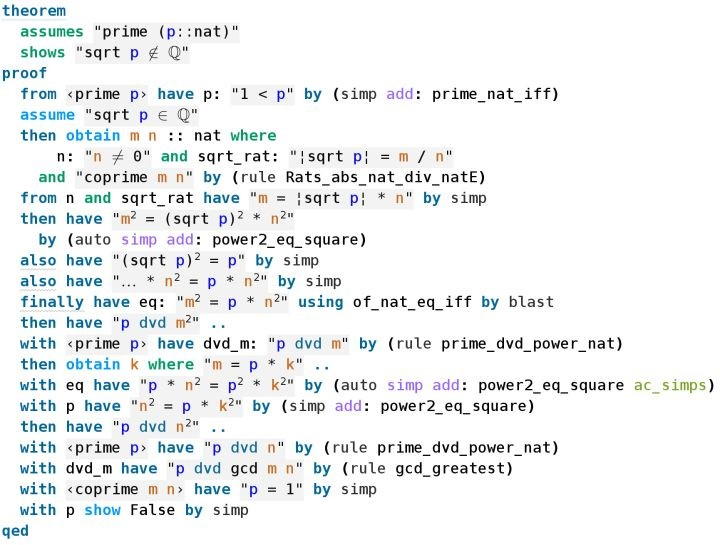
\includegraphics[width=0.6\linewidth]{figure/1}
\caption{Isabelle证明器验证数学定理}
\label{fig:1}
\end{figure}
 
但是,由于数学定理的形式化证明因其过度的复杂性和晦涩的机器表达力,形式化方法没有在数学领域广泛采用\cite{math}。

\subsection{计算机领域的形式化}
\subsubsection{硬件设计领域}
形式化方法在计算机领域是从硬件设计开始普及的,一个例子:当年Intel的Pentium CPU浮点运算单元出错(FDIV Bug),数以万计的CPU不得不回收和替换,给Intel造成了巨大损失(475M美元)。从那之后,Intel开始在其芯片设计中广泛采用形式化方法\cite{verification}。

\subsubsection{软件可靠性方法}
形式化方法在计算机领域最常用的就是软件工程中的形式化方法,又称软件可靠性方法,一般提起形式化方法,往往指的就是计算机领域的软件形式化方法。

从广义上讲,形式化方法是借助数学的方法来解决软件工程领域的问题,主要包括建立精确的数学模型以及对模型的分析活动。狭义的讲,形式化方法是运用形式化语言,进行形式化的规格描述、模型推理和验证的方法。就形式化建模而言,形式化表示必须包含一组定义其语法语义的形式化规则。这些规则可用于分析给定的表达式是否符合语法规定,或证明该表达式具有某种性质。

形式化方法的出发点是数学逻辑方法,其目的是开发可靠的软件产品。从软件开发来讲,形式化方法目前并非软件开发的主流。从软件发展看,早期的软件是用于数值计算,程序语言侧重于函数和算法的描述,后来数据库的应用和数据结构逐渐变得重要。现在的软件更为复杂,因此,对象、组件、接口、通讯、开放等成为非常重要的概念。从软件工程方法来讲,有一套描述这些概念的办法,比如说用图形、表格、逻辑、自然语言等,交叉使用以描述一个系统的各个方面。因此换一个角度来考虑,我们也可以以目前常用的软件开发方法为出发点,研究怎样将这些方法形式化,使软件系统的描述精确化,以减少可能的误解所带来的问题;或以目前常用的软件开发过程为出发点,研究怎样在软件开发过程中增加一些形式化方法的应用,以提高软件的可靠性\cite{1}。

\subsection{协议领域的形式化}
安全协议的形式化分析主要包含:


\subsubsection{安全协议的形式化验证(formal verification)}
对已经存在的安全协议进行验证,判断这些安全协议是否达到预期的目标。本论文的下一章节详细介绍了安全协议的形式化验证技术。

\subsubsection{安全协议的形式化设计(formal design)}
最初人们设计密码协议主要是采用非形式化的方法,由有经验的研究人员根据实际需求设计一些满足特定应用环境的安全协议。事件证明,几乎所有这样设计出的协议都存在安全漏洞。形式化分析方法在成功地发现许多协议漏洞的同时,也不断为协议设计者总结了很多设计经验,如Adnerson和Needham提出的一些健壮性原则,Abadi和Needham提出的理想协议设计规则。但这些规则和经验性原则都是非形式化的,即使协议满足全部的规则,也不能完全保证协议是安全的,于是,形式化的方法也逐渐地应用与协议设计方面。

目前形式化协议设计的思路主要有两种。

一种是研究用于设计协议的方法学,采用这种特定的方法学设计完成后的安全协议可以方便地进行形式化分析,如模块化方法和Fail-Stop协议概念等。模块化方法采用安全推理工具和构成定理(Composition Theorem)得出将两个协议合并为一个安全密码协议的充分条件,当条件不满足时,给出的新协议可能并不安全。Fail-Stop协议的原则就是在一条消息受到攻击时,该消息的所有后继都停止发送,这就保证了攻击不会对外部环境造成影响。另外,Fail-Stop协议的安全性分析比较简单,只需要证明协议在被动攻击下是安全的即可。

另一种协应用更为广泛的设计思路是层次化设计方法,它相当于一个由多种抽象模型形成的堆栈,栈顶是协议设计者根据协议安全性能提出的协议抽象模型,协议设计的过程就是将该抽象模型逐层细化,直到最后得到协议的精确描述或者确切的代码。在协议设计思想的基础上,产生了一些新的协议设计的方法,如Rudolph利用Asynchronous Product Automata设计新的安全协议,Buttyan扥更实用管道的概念进行安全协议设计等。另外,Guttman等人使用认证测试方法,以串空间模型为基础提出了一种用于协议设计的方法。

虽然形式化的方法在协议设计中取得了一定的成果,但是还没有形成完整、有效地理论模型。
\newpage
\section{安全协议的形式化分析方法}
安全协议的形式化分析从方法上可以分为:逻辑推理、模型检测、定理证明。

\subsection{模态逻辑技术}
为了对安全协议进行形式化逻辑推理,必须先对安全协议所涉及的各种对象、状态和关系等进行逻辑抽象。逻辑抽象的作用就是将针对安全性质的讨论放在与算法的数学细节无关的层次上进行,以便于直接理解安全问题的核心,展现问题的逻辑本质。不同形式化框架之间的差别也正是在于逻辑抽象的不同\cite{book}。

模态逻辑分析方法是基于知识与信念推理的分析方法,主要包括信仰逻辑方法和知识逻辑方法,运用逻辑系统从用户接受和发送的消息出发,通过一系列的推理公推证协议是否满足安全规范。逻辑系统是由响应的逻辑语言和推理规则组成的,语言用来描述命题,表示主体对消息的信念和知识,应用推理规则可以从已知的信念或知识推导出新的信念和知识。\cite{book}\cite{2}。

模态逻辑方法是分析安全协议最直接,最简单的一种方法,它的基本思想是:

\begin{enumerate}[(1)]
\item 在安全协议执行前,主体拥有的初始信念或知识。
\item 安全协议的执行过程时主体之间传递信念或知识的过程。随着协议的逐步执行,主体可以通过设定好的推理规则不断从已知的信念或知识推导出新的信念或知识。
\item 安全协议需要验证的安全属性也表示为主体的信念或知识,称为“目标信念或目标知识”。
\item 验证安全协议是否满足所需的安全属性,就等价于安全协议执行完毕时,主体能否从初始信念或知识推导出目标信念或目标知识。所以模态逻辑验证是一个演绎推理的过程。
\end{enumerate}

依照模态逻辑方法的基本思想,这种方法的验证过程为如下几步:

\begin{enumerate}[(1)]
\item 对所需要的规则和公理进行形式化描述。
\item 用逻辑语言形式化地说明协议的步骤。
\item 形式化地描述协议的预期目标(也就是需要验证的安全属性)。
\item 从最初的协议假设开始,运用逻辑公理和推导规则对协议的每一步进行逻辑声明。
\item 将得到的逻辑声明与协议的预期目标进行比较,看是否一致,由此来确定协议是否满足安全属性。
\end{enumerate}

1989年,Burrows,Abadi和Needham提出了著名的BAN逻辑,这种逻辑利用知识和信念逻辑来描述和推理认证协议,通过协议理想化、初始嘉定确定、断言确定和逻辑推理等步骤,验证协议的人整形目标。它简单,直观,便于掌握和使用,是安全协议形式化分析研究中的一个重要的里程碑\cite{2}。

但是,BAN逻辑也有缺陷,它的语义不够精确、协议理想化和初始假设的确定非形式化、推理规则不够完备等,只能验证认证性质,不能认证机密性等其他安全性等\cite{2}。

为了克服BAN逻辑的不足,之后又出现多种BAN类逻辑,如GNY、AT、VO、SVO和MB等逻辑,这些扩展的BAN类逻辑语义更加精确,且根据具体使用情况,学者们还提出了一些专用逻辑,用于分析特定的协议,使这种方法能够支持复杂的安全协议验证,能够检测BAN逻辑无法检测的攻击,应用十分广泛,但都没有原始的BAN逻辑简单实用。


\subsubsection{BAN逻辑}
BAN逻辑以及类BAN逻辑都是基于信仰的逻辑。
\paragraph{基本术语}\

BAN逻辑的处理对象包括主体(Principals)、密钥(Keys)和公式或命题(Formula or Statement)。一般用P、Q、R表示主体变量,K表示密钥,X、Y表示公式变量,并通过角标的形式来表达共享密钥或者公私钥,N表示随机数,h(X)表示hash函数。

除了变量表达,BAN逻辑还包含一系列语法构件。

P$\lvert\equiv$ X:P相信X,即主体P相信命题X是正确的。

P$\triangleleft$X:P看到X,即主体P接收到了包含X的消息,P能读出并重复。

P$\lvert\sim$X:P曾今说过X,即P曾今发送过一条包含X的消息,并且在发送时,P是相信X的。

P$\lvert\Rightarrow$X:P对X有仲裁权,即P对命题X具有权威性,别的主体对此都信服。

\#(X):X是新鲜的,即X是本轮协运行过程中产生的新鲜的随机数。

P$\stackrel{K}{\longleftrightarrow}$Q:K是P与Q的共享密钥,并且除了P、Q以及他们所信任的主体之外,其他主体都不知道该密钥。

$\stackrel{K}{\mapsto}$P:P的公钥为K,且除了P以及他所信任的主体之外,其他主体都不知道其对应的私钥$K^{-1}$。

P$\stackrel{K}{\rightleftharpoons}$P:X为P和Q的共享秘密,且除了P和Q以及他们所信任的主体之外,其他主体都不知道X。

$\{X\}_{K}$:用密钥K加密X后得到的密文。

$<X>_{Y}$:消息X和秘密Y的级联。这里主要是利用Y来证明发出消息$<X>_{Y}$的主体的身份。

\paragraph{推理规则}\

BAN逻辑共有7类19条推理规则。

\begin{enumerate}[(1)]
\item 消息意义规则

消息意义规则共有3条,其目的是从加密消息所使用的密钥以及所包含的秘密来判断消息发送者的身份。

$R_{1}$:$\dfrac{P{\lvert\equiv}Q\stackrel{K}{\longleftrightarrow}P\textrm{,}P\triangleleft\{X\}_{K}}{P{\lvert\equiv}Q{\lvert\sim}X}$

$R_{1}$表明:如果P相信K为P和Q的共享密钥,且P接收到用K加密的X 的密文消息$\{X\}_{K}$,则P相信Q曾发送过消息X。

$R_{2}$:$\dfrac{P{\lvert\equiv}\stackrel{K}{\mapsto}Q\textrm{,} P\triangleleft\{X\}_{K^{-1}}}{P{\lvert\equiv}Q{\lvert\sim}X}$

$R_{2}$表明:如果P相信K是Q的公钥,并且P曾今收到用私钥加密的消息X,那么P相信Q曾今发送过消息X。

$R_{3}$:$\dfrac{P{\lvert\equiv}Q\stackrel{Y}{\rightleftharpoons}P\textrm{,} P\triangleleft\{X\}_{Y}}{P{\lvert\equiv}Q{\lvert\sim}X}$

$R_{3}$表明:如果P相信Q和他共享秘密Y,并且P曾今收到过用Y加密的消息X,那么P相信Q发送过消息X。

\item 随机数验证规则

$R_{4}$:$\dfrac{P{\lvert\equiv}\#(X)\textrm{,} P{\lvert\equiv}Q{\lvert\sim}X}{P{\lvert\equiv}Q{\lvert\equiv}X}$

$R_{4}$表明:如果P相信消息X是新鲜的,且P相信Q曾经发送过X,那么P相信Q相信X。

\item 仲裁规则

$R_{5}$:$\dfrac{P{\lvert\equiv}Q{\lvert\Rightarrow}X\textrm{,} P{\lvert\equiv}Q{\lvert\equiv}X}{P{\lvert\equiv}X}$

$R_{5}$表明:如果P相信Q对X有仲裁权利,并且P相信Q相信X,那么P也相信X。

\item 信仰规则

$R_{6}$:$\dfrac{P{\lvert\equiv}X\textrm{,} P{\lvert\equiv}Y}{P{\lvert\equiv}(X,Y)}$

$R_{7}$:$\dfrac{P{\lvert\equiv}(X,Y)}{P{\lvert\equiv}X}$

$R_{8}$:$\dfrac{P{\lvert\equiv}Q{\lvert\equiv}(X,Y)}{P{\lvert\equiv}Q{\lvert\equiv}X}$

$R_{9}$:$\dfrac{P{\lvert\equiv}Q{\lvert\sim}(X,Y)}{P{\lvert\equiv}Q{\lvert\sim}X}$

$R_{6}$ - $R_{9}$反应了信仰在消息的级联与分割的不同操作中具有一致性和传递性。

\item 消息接收规则

$R_{10}$:$\dfrac{P{\triangleleft}(X,Y)}{P{\triangleleft}X}$

$R_{11}$:$\dfrac{P{\triangleleft}(X)_Y}{P{\triangleleft}X}$

$R_{10}$和$R_{11}$表明如过P接收到了一个级联的消息,那么他可以从中读出子消息。

$R_{12}$:$\dfrac{P{\lvert\equiv}Q\stackrel{K}{\longleftrightarrow}P\textrm{,}P\triangleleft\{X\}_{K}}{P{\triangleleft}X}$

$R_{13}$:$\dfrac{P{\lvert\equiv}\stackrel{K}{\mapsto}Q\textrm{,} P\triangleleft\{X\}_{K}}{P{\triangleleft}X}$

$R_{14}$:$\dfrac{P{\lvert\equiv}\stackrel{K}{\mapsto}Q\textrm{,} P\triangleleft\{X\}_{K^{-1}}}{P{\triangleleft}X}$

$R_{12}$-$R_{14}$表明:如果P收到了一条生命,且P知道相关的密钥,则P可读出消息原文。

\item 消息新鲜性规则

$R_{15}$:$\dfrac{P{\lvert\equiv}\#(X)}{P{\lvert\equiv}\#(X,Y)}$

$R_{15}$表明:如果P相信X是新鲜的,则不论X与任何其他消息级联,整个消息都是新鲜的。

\item 密钥与秘密对称规则

$R_{16}$:$\dfrac{P{\lvert\equiv}R\stackrel{K}{\longleftrightarrow}R'}{P{\lvert\equiv}R'\stackrel{K}{\longleftrightarrow}R}$

$R_{17}$:$\dfrac{P{\lvert\equiv}Q{\lvert\equiv}R\stackrel{K}{\longleftrightarrow}R'}{P{\lvert\equiv}Q{\lvert\equiv}R'\stackrel{K}{\longleftrightarrow}R}$

$R_{18}$:$\dfrac{P{\lvert\equiv}R\stackrel{K}{\rightleftharpoons}R'}{P{\lvert\equiv}R'\stackrel{K}{\rightleftharpoons}R}$

$R_{19}$:$\dfrac{P{\lvert\equiv}Q{\lvert\equiv}R\stackrel{K}{\rightleftharpoons}R'}{P{\lvert\equiv}Q{\lvert\equiv}R'\stackrel{K}{\rightleftharpoons}R}$

\end{enumerate}

\paragraph{BAN逻辑分析具体协议的示例}\

本节将结合Needham-Schroeder对称密钥协议说明BAN逻辑的分析过程,BAN逻辑的分析过程如下: 

\begin{itemize}
\item 协议的形式化描述
\item 定义初始化假设
\item 定义协议目标
\item 应用推理规则对协议进行推理和验证
\end{itemize}

BAN逻辑协议形式化分析流程如图(\ref{fig:3})所示。

\begin{figure}[h!]
\centering
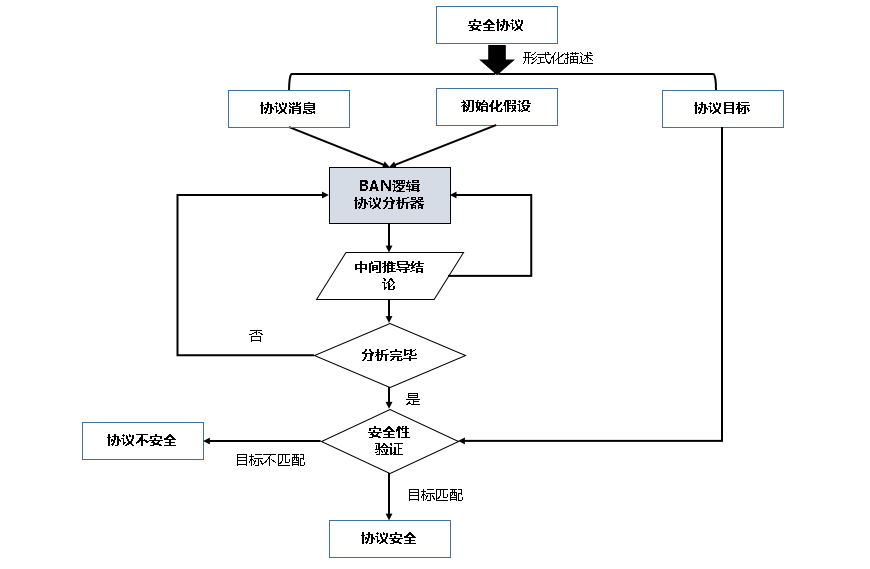
\includegraphics[width=0.8\linewidth]{figure/3}
\caption{BAN逻辑协议形式化分析流程}
\label{fig:3}
\end{figure}

\subparagraph{Needham-Schroeder协议过程}\

该协议涉及3个主体,通信双方A,B以及他们都信赖的认证服务器S。其中,$K_{AS}$是A与S之间的共享密钥,$K_{BS}$是B与S之间的共享密钥,$K_{AB}$是A、B双方的会话密钥,由S生成,$N_{A}$和$N_{B}$分别是由A和B生成的随机数。该协议的目标是使通信双方能够互相证实对方的身份,并且为后续的加密通信建立一个会话密钥。协议的过程如下:

\begin{enumerate}[(1)]
\item A$\to$S:A,B,$N_{A}$
\item S$\to$A:${\{N_{A},B,K_{AB},{\{K_{AB},A\}}_{K_{BS}}\}}_{K_{AS}}$
\item A$\to$B:${\{K_{AB},A\}}_{K_{BS}}$
\item B$\to$A:${\{N_{B}\}}_{K_{AB}}$
\item A$\to$B:${\{N_{B}-1\}}_{K_{AB}}$
\end{enumerate}

BAN逻辑可以分析出该协议具有的重放攻击漏洞,过程如下。

\subparagraph{协议的形式化描述(理想化过程)}\

$M_{1}$忽略,因为是明文传递,与安全属性的分析无关。

$M_{2}$:S$\to$A: ${\{N_{A},(A\stackrel{K_{AB}}{\longleftrightarrow}B),\#(A\stackrel{K_{AB}}{\longleftrightarrow}B),{(A\stackrel{K_{AB}}{\longleftrightarrow}B)}_{K_{BS}}\}}_{K_{AS}}$

$M_{3}$:A$\to$B:$ {A\stackrel{K_{AB}}{\longleftrightarrow}B)}_{K_{BS}}$ 

$M_{4}$:B$\to$A:${\{N_{B},(A\stackrel{K_{AB}}{\longleftrightarrow}B)\}}_{K_{AB}}$ from B

$M_{4}$:A$\to$B:${\{N_{B},(A\stackrel{K_{AB}}{\longleftrightarrow}B)\}}_{K_{AB}}$from A

\subparagraph{初始化假设}\

关于密钥的有效性的假设:

$A_{1}$: $A{\lvert\equiv}A\stackrel{K_{AS}}{\longleftrightarrow}S$

$A_{2}$: $B{\lvert\equiv}B\stackrel{K_{BS}}{\longleftrightarrow}S$

$A_{3}$: $S{\lvert\equiv}A\stackrel{K_{AS}}{\longleftrightarrow}S$

$A_{4}$: $A{\lvert\equiv}B\stackrel{K_{BS}}{\longleftrightarrow}S$

$A_{1}$: $S{\lvert\equiv}A\stackrel{K_{AB}}{\longleftrightarrow}B$

关于S的可信性:

$A_{6}$: $A{\lvert\equiv}(S{\lvert\Rightarrow}A\stackrel{K_{AB}}{\longleftrightarrow}B)$

$A_{7}$: $B{\lvert\equiv}(S{\lvert\Rightarrow}A\stackrel{K_{AB}}{\longleftrightarrow}B)$

$A_{8}$: $A{\lvert\equiv}(S{\lvert\Rightarrow}\#(A\stackrel{K_{AB}}{\longleftrightarrow}B))$

$A_{8}$表明:A相信S所生成的会话密钥同时具有随机数的性质,因为一个”好“的加密密钥通常具备随机数的特征。

关于随机数的新鲜性:

$A_{9}$: $A{\lvert\equiv}\#(N_{A})$

$A_{10}$: $B{\lvert\equiv}\#(N_{B})$

$A_{11}$: $S{\lvert\equiv}(A\stackrel{K_{AB}}{\longleftrightarrow}B)$

$A_{12}$: $B{\lvert\equiv}(A\stackrel{K_{AB}}{\longleftrightarrow}B)$

\subparagraph{协议目标的形式化描述}\

$G_{1}$: $A{\lvert\equiv}A\stackrel{K_{AB}}{\longleftrightarrow}B$

$G_{2}$: $B{\lvert\equiv}A\stackrel{K_{AB}}{\longleftrightarrow}B$

$G_{3}$: $A{\lvert\equiv}B{\lvert\equiv}A\stackrel{K_{AB}}{\longleftrightarrow}B$

$G_{3}$: $B{\lvert\equiv}A{\lvert\equiv}A\stackrel{K_{AB}}{\longleftrightarrow}B$

\subparagraph{逻辑推理以及验证}\

由$M_{2}$可知,$A\triangleleft{\{N_{A},(A\stackrel{K_{AB}}{\longleftrightarrow}B),\#(A\stackrel{K_{AB}}{\longleftrightarrow}B),{(A\stackrel{K_{AB}}{\longleftrightarrow}B)}_{K_{BS}}\}}_{K_{AS}}$ ,即A看到了S发送的由$K_{AS}$加密的$N_{A}$等信息,又由初始化假设$A_{1}$,应用消息意义规则$R_{1}$可得

\begin{equation}
A{\lvert\equiv}S{\lvert\sim}(N_{A},A\stackrel{K_{AB}}{\longleftrightarrow}B,\#(A\stackrel{K_{AB}}{\longleftrightarrow}B),{(A\stackrel{K_{AB}}{\longleftrightarrow}B)}_{K_{BS}})
\end{equation}

即A相信S曾今发送过这些消息。

再由初始化假设$A_{9}$,应用随机数验证规则$R_{4}$,可得

\begin{equation}
A{\lvert\equiv}S{\lvert\equiv}(N_{A},A\stackrel{K_{AB}}{\longleftrightarrow}B,\#(A\stackrel{K_{AB}}{\longleftrightarrow}B),{(A\stackrel{K_{AB}}{\longleftrightarrow}B)}_{K_{BS}})
\end{equation}

即A信任S相信这些信息的正确性。

应用信仰规则$R_{7}$可得

\begin{equation}
A{\lvert\equiv}S{\lvert\equiv}A\stackrel{K_{AB}}{\longleftrightarrow}B,{\quad}A{\lvert\equiv}S{\lvert\equiv}\#(A\stackrel{K_{AB}}{\longleftrightarrow}B)\label{e1}
\end{equation}

即A信任S信任$K_{AB}$是A和B的共享密钥,A也信任S信任上述知识是新鲜的。

由初始化假设$A_{6}$、$A_{8}$以及式(\ref{e1}),应用仲裁规则$R_{5}$可得

\begin{equation}
A{\lvert\equiv}A\stackrel{K_{AB}}{\longleftrightarrow}B,{\quad}A{\lvert\equiv}\#(A\stackrel{K_{AB}}{\longleftrightarrow}B)\label{e2}
\end{equation}

A信任$K_{AB}$是A和B的共享密钥,A信任此知识是新鲜的。

由$M_{3}$可知,$B\triangleleft{(A\stackrel{K_{AB}}{\longleftrightarrow}B)}_{K_{BS}}$即B曾今看到过由$K_{BS}$加密后的$K_{AB}$,由初始化假设$A_{2}$,应用消息意义规则$R_{1}$,可得

\begin{equation}
B{\lvert\equiv}S{\lvert\sim}A\stackrel{K_{AB}}{\longleftrightarrow}B
\end{equation}

即B信任S曾今发送过A和B的共享密钥$K_{AB}$。

再由初始化假设$A_{12}$,应用随机数验证规则$R_{4}$,可得

\begin{equation}
B{\lvert\equiv}S{\lvert\equiv}A\stackrel{K_{AB}}{\longleftrightarrow}B
\end{equation}

即B信任S信任$K_{AB}$是A和B的共享密钥。

再由初始化假设$A_{7}$,应用仲裁规则$R_{5}$,可得

\begin{equation}
B{\lvert\equiv}A\stackrel{K_{AB}}{\longleftrightarrow}B\label{e3}
\end{equation}

即B信任$K_{AB}$是A和B的共享密钥。

通过$M_{4}$和$M_{5}$,主体A、B均确信对方在线,再由$M_{4}$可知

\begin{equation}
A\triangleleft{\{N_{B},(A\stackrel{K_{AB}}{\longleftrightarrow}B)\}}_{K_{AB}}{\quad}from B
\end{equation}

即A曾今见到过由B发送的,通过$K_{AB}$加密的$N_{B}$和$K_{AB}$

由式(\ref{e2})中的$A{\lvert\equiv}A\stackrel{K_{AB}}{\longleftrightarrow}B$,应用消息意义规则$R_{1}$,可得

\begin{equation}
A{\lvert\equiv}B{\lvert\sim}(N_{B},A\stackrel{K_{AB}}{\longleftrightarrow}B)
\end{equation}

即A信任B曾今发送过$N_{B}$和$K_{AB}$

再由信仰规则$R_{9}$可得

\begin{equation}
A{\lvert\equiv}B{\lvert\sim}(A\stackrel{K_{AB}}{\longleftrightarrow}B)
\end{equation}

即A信任B发送过$K_{AB}$

再由式(\ref{e2})中的$A{\lvert\equiv}\#(A\stackrel{K_{AB}}{\longleftrightarrow}B)$,根据随机数验证规则$R_{4}$可得

\begin{equation}
A{\lvert\equiv}B{\lvert\equiv}A\stackrel{K_{AB}}{\longleftrightarrow}B\label{e4}
\end{equation}

即A信任B信任$K_{AB}$是A和B的共享密钥。

同样,由$M_{5}$可知,$B\triangleleft{\{N_{B},(A\stackrel{K_{AB}}{\longleftrightarrow}B)\}}_{K_{AB}}$,B曾看到过A发送的,用$K_{AB}$发送的$N_{B}$和$K_{AB}$,经过类似推理,可得

\begin{equation}
B{\lvert\equiv}A{\lvert\equiv}A\stackrel{K_{AB}}{\longleftrightarrow}B\label{e5}
\end{equation}

即B信任A信任$K_{AB}$是A和B的共享密钥。

由上述推导过程中的式(\ref{e2})、式(\ref{e3})、(\ref{e4})和式(\ref{e5})可知,在12个假设均满足的情况下,协议达到了预期目标。而为了验证协议满足目标$G_{2}$,必须借助于初始化假设$A_{12}$,即B相信会话密钥$K_{AB}$是新鲜的,而这一假设是不合理的,因为B无从获得$K_{AB}$是否新鲜,因此该协议可能受到重放攻击。\vspace{12pt}

BAN逻辑的不足主要表现在它逻辑的抽象级别较高,分析范围过窄,不能对知识进行推理,只能分析协议的认证性质,只能发现协议的缺陷,不能保证协议一定是安全的\cite{4}。

\begin{itemize}
\item 协议的理想化过程不规范。
\item 协议的初始化假设不合理。
\item 缺乏完备性。
\item 缺乏一个定义良好、确切的语义。
\end{itemize}

\subsubsection{类BAN逻辑}

因为BAN逻辑存在着上节提出的诸多问题,所以人们尝试改进BAN逻辑,由此产生了多种类BAN逻辑,如GNY、AT、VO、SVO和MB等逻辑等。

\paragraph{GNY逻辑}

GNY逻辑是第一个对BAN进行增强扩充的逻辑,它试图消除BAN逻辑中对主题城市性的假设、消息源假设和可识别假设,并从以下方面对BAN逻辑进行了改进。

\begin{itemize}
\item 增加了新的逻辑构件和规则,推广了逻辑分析的应用范围,使之能分析某些具有单向函数的密码协议。
\item 取消了全局假设,增强了逻辑分析能力。
\item 理想化协议时保留了明文
\item 增加了“拥有”集合,即主体能看到的所有符号的集合。
\item 引入“可识别性”概念,可以描述主体对其所期望的消息格式的识别能力。
\item 引入了“不是由此首发”的识别机制,来判断消息的来源,取消了BAN逻辑中主体能识别协议消息来源的假设。
\end{itemize}

\paragraph{AT逻辑}
与GNY逻辑类似,均对BAN逻辑的本质与局限性进行了分析与改进。不同的是,AT逻辑首次提出了逻辑系统的语义模型,表达能力更强。

\paragraph{SVO逻辑}
VO逻辑的目的是扩展BAN逻辑的应用范围,比如,增加了分析Diffie-Hellman协议的能力,进而可以分析Internet密钥交换协议IKE和SSL协议等。VO逻辑还细化了认证协议的认证目标,给出了6种不同形式的认证目标,包括Ping认证、实体认证、安全密钥的建立、密钥确认、密钥新鲜性认证和共享密钥的互信任等。

SVO逻辑在总结BAN逻辑、GNY逻辑、AT逻辑以及VO逻辑的基础上发展而成,具有相当详细的计算模型,具有几号的扩展能力,简介、易用,标志着BAN逻辑以及BAN类逻辑的成熟。

\paragraph{Kailar逻辑}
随着电子商务协议的出现,一些新的安全协议的心智引起了人们的密切关注,如不可否认性和可追究性等安全属性。Kailar逻辑恰恰是针对此类安全属性而开发的形式化分析工具。

\subsubsection{基于知识的逻辑}

人们发现,BAN逻辑以及类BAN逻辑都是基于主体信仰的,一个主要问题在与主体的信仰有可能是错误的,而他本人可能并不知道该信仰是错误的。基于错误的信仰并不能保证协议的安全性。为此,P.Bieber基于CKT5认知逻辑,提出了一套基于知识的安全协议分析逻辑。认知逻辑最早由Hintikka与1962年提出,1984年,Halpern和Moses将其成功地应用于分布式系统的分析中。CKT5认知逻辑对认知逻辑进行了补充,从而能描述在敌对环境中利用加密消息进行通信的各主体的知识状态。

\subsubsection{非单调逻辑}

前面介绍的逻辑分析方法都是针对知识和信仰的单调推理逻辑,即一旦主体知道了某些事情或者拥有了某些信仰,他就永远知道这些事情或者拥有这些信仰。这在某些情况下是不适用的。例如,如果某一会话密钥被泄露了,那么该密钥是“好密钥”的信仰就要被改变,不再成立。为此,Moser提出了一种针对信仰的非单调推理逻辑,但不能处理非单调的知识。Rubin博士提出了一个分析安全协议的新方法,用以非单调地分析密码协议,这种分析方法称为非单调(Nonmonotomic)逻辑分析方法。

\subsection{模型检测技术(model checking)}

模型检测最早用于分析和模拟硬件的工作过程。1996年,Gavin Lowe首次将模型检测器FDR(Failures-Divergences Refinement:故障发散提炼器)用于安全协议的验证,结合CSP安全协议模型成功发现了针对NSPK协议的攻击,此后,又出现了NRL(Naval Research Laboratory)协议分析器,Interrogator系统,CSP/FDR模型检测器,Brutus模型检测器,SMV,MUφ,SPN,Athena,OFMC,SATMC等大量自动化验证器\cite{1}\cite{5}\cite{6}。

模型检测技术的安全协议分析方法也称为状态检测方法。主要利用有限状态机的理论,通过状态空间搜索方法来检测协议安全性,其基本思想是将安全协议看做包含一个状态集合、一个动作集合、一个状态转移集合的分布式系统。协议的执行过程就是状态的迁移过程,协议验证就是遍历整个状态空间,检查是否能由初试的状态到达某个不安全状态或者可以引发某个不良行为的状态。初始状态到最终状态之间的所有状态构成了一个协议执行轨迹,如果一个协议不安全,就可以通过协议迹给出相应的反例\cite{2}\cite{6}。

\cite{book}中提到,模型检测方法应用于安全协议分析的基本思想是:把安全协议看成一个分布式系统,单个主体涉及的协议执行部分称为局部状态,所有局部状态构成系统的全局状态;在协议执行过程中,主体收发消息的动作会引起局部状态的改变,进而也引起全局状态的改变;在安全协议全局状态上定义安全属性或不变关系,则安全协议是否满足安全目标等价于在系统可达的每个全局状态上安全属性或不变关系是否都能得到满足。

模型检测分析方法取得了很大的成功,对于目前的协议分析来讲,模型检测已经证明是一条非常成功的途径,这种方法的自动化程度高,验证过程不需要用户参与,而且如果协议有缺陷,能够自动产生反例。但是缺点也很明显,就是容易产生状态空间爆炸,一般需要制定运行实例和主体数量等运行参数。同时,在无限状态模型中,模型检测无法完全确定协议是安全的\cite{1}。

对于该方法面临的''状态空间爆炸问题'',可以通过控制状态空间大小,控制搜索过程的手段来解决。不同的模型检测器都有着相关的技术来解决这一问题,例如,Clarke等使用偏序规约技术削减状态空间以解决状态空间爆炸问题;Huima第一次采用符号技术来解决无限状态空间搜索的问题;Lowe探讨了模型检测方法的完备性问题,证明在一定条件下,如果一个小系统是安全的,那么大系统也是安全的。

常用的模型检测技术包括有限状态机、Petri网和通信进程演算(Cacula for Communication System, CCS)。

\subsubsection{Dolev-Yao模型}
模型检测方法和定理证明方法大多是基于Dolev-Yao模型的,故本节先对Dolev-Yao模型进行介绍。

该模型是由Dolev、Yao与1983年首次提出的安全协议形式化分析的假设和模型,分别刻画了密码系统模型以及攻击者模型。

\paragraph{密码模型}
密码系统模型将密码系统看做是一个黑盒子,并假设采用的密码算法和密码技术是完善的;主体仅在拥有了正确的解密密钥时才能进行解密,并且产生的密文必须拥有对应的明文和加密密钥。这就使得攻击者无法进行密码分析,从而将安全协议本身与安全协议所采用的密码系统分开考虑,降低了安全协议分析问题的复杂度,

\paragraph{攻击者模型}
攻击者模型描述了攻击者的知识和能力,具体包括如下几个方面。

\begin{enumerate}[(1)]
\item 熟悉现代密码学,知道加解密等运算操作。
\item 知道参与协议运行的各个实体以及其公钥。
\item 拥有自己的加密密钥和解密密钥,并且能够将窃听或收到的消息增加为自己的新知识。
\item 对网络具有完全的控制能力,可以窃听。拦截系统中传送的所有消息。
\item 可以用他拥有的加密或者解密密钥对消息进行加解密操作。
\item 可以在系统中插入新的消息。
\item 即使不知道加密部分的内容,他也可以重放他所看到的任何消息。
\item 可以生成新的随机数。
\end{enumerate}

Dolev-Yao模型中的攻击者非常强大,这使得在分析安全协议时,可以使安全协议经手极其恶劣的网络环境的考验而确保其安全属性成立,但是,该模型下,无法对所使用的密码系统的缺陷进行分析,从而使得由该模型建立的形式化分析方法无法用于分析安全协议密码系统相关的缺陷攻击和猜测攻击,同时,Dolev-Yao模型下攻击者的能力太强,攻击者总能实现拒绝服务攻击,这又和现实情况相违背。
\subsubsection{有限状态机}
有限状态机,又称有限状态自动机,是表示有限个状态以及在这些状态之间转移和动作等行为的数学模型。

有限状态机在不同领域中都很重要,在计算机科学中,有限状态机被用于建模应用行为、硬件电路系统设计、软件工程、编译器、网络协议和计算与语言的研究。

有限状态机是描述协议常用的模型,可以用有向图直观地表示协议的模型。通常,将协议有限状态机模型定义为一个四元祖M:

\begin{equation}
M=\{S,i,e,T\}
\end{equation}

其中,S是模型中协议所有状态的又穷集合,即系统状态机;i为系统初始状态的有穷集合,i$\in$S,T为状态转换函数的有穷集合,定义系统的状态转换规则,转换函数定义为$s_{i}\stackrel{e}{\longrightarrow}s_{j}\in{T},s_{i}\in{S},S_{j}\in{S},e\in{E}$,表示当系统属于状态$s_{i}$时,如果有事件e,那么系统状态就变为$s_{j}$

\subsubsection{通信进程方法}
通信进程演算的数学基础是进程代数,由R.Miller创立的通信进程演算已经在协议工程领域得到了重要应用,C.A.Hoare在CCS的基础上创立了通信顺序进程。通信顺序进程(Communicating Sequential Process, CSP)是一种用来描述并发系统中通过消息交互的通信实体行为的抽象符号语言。这种方法能够用来描述和分析由很多进程构成的系统,进程之间通过消息交换而相互作用。

CSP方法在安全协议的分析验证方面得到了成功的应用,主要步骤是将安全协议的信息交互规约为CSP,将其安全目标也在CSP框架内描述为CSP要说明的问题,然后通过有效地分析方法对这些描述进行推理。目前,FDRC(Failures-Divergences Refinement:故障发散提炼器)是比较有代表性的自动化模型检测器。

\paragraph{CSP的基本概念}
\subparagraph{事件}\

协议是通过实体之间执行一系列的事件(Event)来执行的,一个典型的CSP事件表示为c.i.j.m,其中包括一个信道c、一个消息源i、一个消息目的地j、一个消息m。

\subparagraph{进程}\

CSP通过用某一进程(Processes)可能涉及到的事件来描述该进程,从而提供了一种描述进程可达状态的方法。进程通常表示为:执行状态中的一个动作(事件)、动作结束后的状态。常用的CSP有:

\begin{enumerate}[(1)]
\item 停止进程 STOP
\item 事件前缀 a$\rightarrow$P,表示执行动作a后按照进程P来执行。
\item 顺序组合 P;Q  表示P结束前只运行P的事件,P结束后才运行Q的事件,并且直到Q终止,P;Q才终止。
\item 输入前缀选择 $c?x:A\rightarrow{P}$,表示在信道c上接受任意输入x$\in$A之后,执行进程P。
\item 输出前缀选择$c!x\rightarrow{P}$,表示在信道c上输出x之后,执行进程P。
\item 进程间选择P$\square$Q,表示在P和Q之间做选择,结果或为P,或为Q。$\square$的作用就是给出了两个进程动作的选择项,然后按照其中一个选择的动作运行。
\item 并行进程P$\parallel$Q,强制所有的事件都是同步的,当P和Q都可以执行时,P$\parallel$Q才可以执行。
\item 接口并行
\item 一般穿插P$\mid\mid\mid$Q,表示P和Q使用分离的事件集合。$\mid\mid\mid$S表示执行S集合中所有进程的并行运行。
\item 同步并行$P_{X}\parallel$$_{Y}Q$表示P与Q并联,并且P和Q的字母表是X和Y,即P一定统一所有X中的通信,Q一定统一所有Y中的通信。
\item 成功终止 SKIP
\item 递归进程$\mu$P.F(P),表示F(P)递归地执行。
\end{enumerate}

\subparagraph{迹}\
一个进程的迹(Traces)模型描述了该进程所有可能的事件序列。

与迹有关的表示如下:

\begin{enumerate}[(1)]
\item tr$\uparrow$D:表示tr中由D中事件组成的最大子序列。
\item tr$\downarrow$C:表示在信道C上传输的最长消息序列。
\item tr$\Downarrow$C:表示在C中某些信道上传输的消息集合。
\item $\delta$(tr):表示在迹tr上出现的事件集合。若将此操作扩展到进程上,则$\delta$(P)表示在进程P的某些迹上出现的事件集合。
\end{enumerate}

迹上的运算规则有:

\begin{enumerate}[(1)]
\item traces(STOP) = $\{\langle\rangle\}$
\item traces(a$\rightarrow$P) = $\{\langle\rangle\}\cup\{\langle{a}\rangle{s}\mid{s}\in{traces(P[a/x])}\}$,即该进程要么什么都不做,要么第一个事件总是a,并且其后有一个P的迹。
\item trace(P$\square$Q)=traces(P)$\cup$traces(Q),该进程提供了P的迹和Q的迹。
\end{enumerate}

\subparagraph{CSP网络模型描述具体的协议}\

下面以Yahalom协议为例,来说明用CSP方法对协议的建模过程。协议内容如下:

$m_{1}$:  A$\rightarrow$B:a.$n_{a}$

$m_{2}$:  B$\rightarrow$S:\{a.$n_{a}.n_{b}\}_{ServerKey(b)}$

$m_{3}$:  S$\rightarrow$A:\{b.$k_{ab}.n_{a}.n_{b}\}_{ServerKey(b)}.\{a.k_{ab}\}_{ServerKey(b)}$

$m_{4}$:  A$\rightarrow$B:\{a.$n_{a}.k_{ab}\}_{ServerKey(b)}.\{n_{b}\}_{k_{ab}}$

该协议参与方有三个,分别是初始者A,响应者B和服务器S。

初始者A的CSP进程描述如下,其中m表示任意的输入m,因为在m3中,A无法对收到的$\{a.k_{ab}\}_{ServerKey(b)}$进行解密,因为A没有ServerKey(b),所以表示成任意输入m是合理的。env?B:Agent是一个表达式,表示进程的局部环境会告诉它如何开放一个与代理B的会话。

\begin{multline}
Initiator(A,n_{a})=env?B:Agent\rightarrow{send.A.B.a.n_{a}}\rightarrow\\
\square{k}_{ab}\in{Key},n_{b}\in{Nonce},\\
m\in{T}\left(
\begin{array}{lr}
	{receive.S.A\{b.k_{ab}.n_{a}.n_{b}\}_{ServerKey(a)}.m}\rightarrow& \\
	{send.A.B.m.\{n_{b}\}_{k_{ab}}}\rightarrow{Session(A,B,k_{ab},n_{a},n_{b})}&
\end{array}
\right)
\end{multline}

同理,响应者的角色进程为:

\begin{multline}
Responder(B,n_{b})=\square{k_{ab}}\in{Key},A\in{Agent} \\
\left(
\begin{array}{lr}
	{receive.A.B.a.n_{a}\rightarrow}& \\
	{send.B.S.b.\{a.n_{a}.n_{b}\}_{ServerKey_{b}}}\rightarrow& \\
	{receive.A.B.\{a.k_{ab}\}_{ServerKey(b)}.\{n_{b}\}_{k_{ab}}\rightarrow}& \\
	{Session(B,A,k_{ab},n_{a},n_{b})})&
\end{array}
\right)
\end{multline}

服务器的CSP进程如下,其中,用一般穿插来保证$k_{ab}$每次不是单个的密钥,而是属于服务器密钥集合的不同密钥。

\begin{multline}
Server(S)={\mid\mid\mid}_{k_{ab}\in{KEYS_{Server}}}Serv(S,k_{ab}) \\
Serv(S,k_{ab})=\square{a},b\in{Agent};n_{a},n_{b}\in{Nonce}\\
\left(
\begin{array}{lr}
	{receive.B.S.b.\{a.n_{a}.n_{b}\}_{ServerKey(b)}}\rightarrow& \\
	{send.S.A.\{B.k_{ab}.n_{a}.n_{b}\}_{ServerKey(a).\{a.k_{ab}\}_{ServerKey(b)}}}\rightarrow& \\
	{Server(S,k_{s})}&
\end{array}
\right)
\end{multline}

因为Yahalom协议中,参与方AB既可以作为初始者,也可以作为响应者,所以统称他们为代理a,一个特定的代理a的CSP描述为:

\begin{equation}
User_{a}=({\mid\mid\mid}_{n\in{Nonce\_I_{a}}}Initiator(a,n))\mid\mid\mid({\mid\mid\mid}_{n\in{Nonce\_R-{a}}}Responder(a,n))
\end{equation}

对于一个有入侵者的网络环境,应当存在一个入侵者进程,它能够偷听、阻止任何一个消息,也可以基于假设产生新的消息,同时也可以冒充其他代理的身份,入侵者的CSP进程表示为:

\begin{multline}
Inruder(X)=learn?m:messages\rightarrow{Intruder(close(X\cup{\{m\}}))}\\
\square{?}m:X\cap{messages}\rightarrow{Intruder(X)}
\end{multline}

结合用户、服务器、入侵者,可以将Yahalom协议进行如下描述:

\begin{equation}
Yahalom=User_{A}\mid\mid\mid{User_{B}}\mid\mid\mid{User_{S}}\mid\mid{Intruder}
\end{equation}

\subsubsection{Pertri网}
Petri网是由伯恩大学的C.A.Petri于1962年提出的一种可表示系统部件异步并发操作的网络模型。Petri往在科研工作中的各个领域得到了广泛的应用,并逐渐发展成为高级Petri网:谓词/变迁系统(Pr/T系统)和颜色Petri网(coloured Petri net,CPN)系统。

Petri网定义为5元系统\{P,T,I,O,M\},其中,P为位置集合,$P=\{P_{1},P_{2},\ldots{P_{i}},\ldots{\}}$;T为转换集;I为输入函数集;O为输出函数集;M为标记集,也是Petri网的状态集合。

Petri网可以用来描述协议的状态。

\subsubsection{通用模型检测器}
通用模型检测器有FDR、SPN、SMV、BRUTUS等。

在建模入侵者模型是,需要规定入侵者知道和不知道的消息,如果消息的数目是无限的,则模型本身也将是无限大的,这样在模型中就必须明确规定哪些信息包含、哪些信息排除,用户的负担是简历一个入侵者的有限状态机描述,这一步相对来说比较复杂,特别是在考虑不同协议之间交互的时候\cite{3}。

\subsubsection{专用模型检测器}
专用模型检测器有NRL、BRUTUS等。

专用模型检测器从模型中分离出入侵者,用户不需要事先规定入侵者必须知道的消息,就可以进行协议验证。但是,专用模型检测器的简约技术不如通用模型检测器,在验证复杂协议时经常由于状态爆炸的问题而难以得到验证结果,或者验证结果过给出的反例过于复杂,难以构建攻击路径。其次,专用模型检测器通常只适用于验证某一类型的协议,或者在描述协议的某些性质和验证协议的某些阶段工作做的较好,而在其他方面则存在明显的缺陷\cite{3}。


\subsection{定理证明技术}
基于定理证明的安全协议分析方法不关注针对协议的攻击,其目的只在于证明安全协议是否满足响应的安全属性。

定理证明的分析方法解决了基于逻辑推理方法不能解决保密性验证,缺乏清晰语义的缺点,还解决了模型检测技术很难解决状态空间爆炸的缺点,可以处理不受限会话数目和不受限消息大小,在此方面Pauson和Blanchet的工作最具有代表性。但是Pauson基于归纳的方法只能实现半自动的协议形式化验证,Blanchet基于归结定理证明实现了秘密性和认证性的自动化验证,其验证器可以保证终止,但是不保证完备性,有攻击误报的情况\cite{6}。

(归结原理:将普通形式逻辑中充分条件的推理形式符号化,并向一阶谓词逻辑推广的一种推理法则。)

\subsubsection{Paulson归纳法}
Pauson首先将归纳法应用于协议安全性证明。Isabelle工具把协议定义为所有可能时间执行轨迹的集合,每个执行序列反映了协议主体之间可能的通信方式。它通过对路径的归纳来证明性质的成立。该工具可以用于一个任意次数的协议会话,其证明股构成与非形式化证明方法有着相同的结构,这是它的有点,但是一旦推导失败,就很难获得协议可能的漏洞,并且分析不保证会终止,且需要大量的用户干预\cite{6}。


\subsubsection{串空间模型(Strand-Space)}
Fabrega等人提出了串空间模型,其中协议的正确性可以表示成不同类型串之间的连接关系。正确性证明的过程首先是建立协议规范可能形成的所有串束,再根据串束中串的连接情况判断协议中的安全属性是否得到满足。

之后,Millen等人将串空间的概念和Pauson的归纳证明方法结合起来,使用归纳方法简历协议时间的执行序列,然后在这个序列上使用''补集(co-ideal)''的概念来分析攻击者的知识,来判断保密消息是否已经泄露。

在串空间模型的基础上,Guttman等人提出了反应随机数在加密条件下与身份认证之间关系的认证测试概念,基于这种认证测试机制,既可以证明认证属性,也可以设计认证协议。

Athena是Song等人开发的专用于协议验证的定理证明器,它使用一种扩展的传空间理论作为底层的计算模型,协议的安全属性由一些公式来描述,然后由Athena系统验证这些公式的正确性。它采用宽度优先搜索,若协议不正确,能及早发现攻击行为。由于该工具基于定理证明方法,用户手动状态约简的操作必不可少,并且过程较为繁琐\cite{6}。

\subsubsection{阶函数(Rank Functions)}
阶函数是另一种定理证明方法,它是Schneider提出的概念。

阶函数是一个把攻击者的知识和协议消息映射成整数的函数。使用阶函数可以把消息分成攻击者知道的消息和攻击者不可知道的消息两大类。协议的认证性和秘密性均基于阶函数的值来判定。

后来,Heather和Schneider又给出了一个简历阶函数的算法和推导消息阶函数值的过程,这使得阶函数的证明过程得以自动化实现\cite{6}。

\section{典型的安全协议形式化分析工具}
\subsection{基于知识与信念的模态逻辑方法的工具}
\subsection{基于模型检测的分析工具}
\subsubsection{FDR(故障偏差精炼检查器)}
FDR(Failures-Divergence Refinement,故障偏差精炼检查器)是指银行总针对有限状态机的模型检查工具,其理论基础是Hoare的CSP(通信顺序进程)并发模型,它通过对一个希望满足某些属性的变迁系统的精炼来验证这些属性是否成立。

早期的FDR只用直观的模型检测技术,在几小时内就能处理约$10^{7}$个状态,但是状态空间随着网络中进程数目呈现指数增长,因此该工具显示出了局限性。

Casper/FDR使用进程代数CSP和模型检测器FDR来分析安全协议,Capser(Complier for the Analysis of Security Protocols)是一个安全协议分析编译器,它能将高级语言协议规范转换为CSP语言,解决了利用CSP描述协议系统费时,易出错的问题。是目前应用十分广泛的一个模型检测器,它在NSPK协议发表17年后检测出了协议的中间人攻击。

Casper/FDR的工作步骤如下:

\begin{enumerate}[(1)]
\item 参与协议的每个主题都用CSP进程表示。
\item 攻击者也用CSP进程表示。
\item 检查系统是否满足安全性质,如认证性、保密性,使用FDR搜索状态空间以发现任何不安全的路径是否存在。
\item 如果FDR发现协议的性质不满足,它将给出性质不满足的路径,这条路径对应协议的一个攻击\cite{1}。
\end{enumerate}

利用Casper/FDR分析安全协议的步骤如图(\ref{fig:4})所示:

\begin{figure}[h!]
\centering
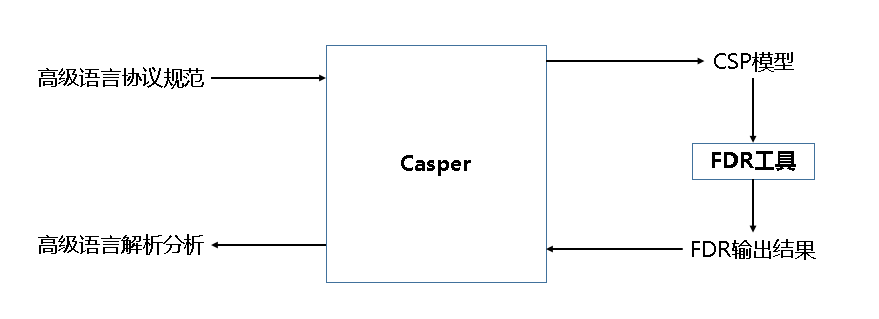
\includegraphics[width=0.8\linewidth]{figure/4}
\caption{Casper/FDR分析安全协议的步骤\cite{1}}
\label{fig:4}
\end{figure}


\section{总结}
未完待续
%============= 参考文献 =====================
\addcontentsline{toc}{section}{参考文献}
\bibliography{bibfile}
\clearpage
%%%%%%%%%% 结束 %%%%%%%%%%
\end{document}